%%%%%%%%%%%%%%%%%%%%%%%%%%%%%%%%%%%%%%%%%%%%%%%%%%%%%%%%%%%%%%%%%%%%%%%%%%%%%%%
%                       CARREGA DE LA CLASSE DE DOCUMENT                      %
%                                                                             %
% Les opcions admissibles son:                                                %
%      12pt / 11pt            (cos dels tipus de lletra; no feu servir 10pt)  %
%                                                                             %
% catalan/spanish/english     (llengua principal del treball)                 %
%                                                                             % 
% french/italian/german...    (si necessiteu fer servir alguna altra llengua) %
%                                                                             %
% listoffigures               (El document inclou un Index de figures)        %
% listoftables                (El document inclou un Index de taules)         %
% listofquadres               (El document inclou un Index de quadres)        %
% listofalgorithms            (El document inclou un Index d'algorismes)      %
%                                                                             %
%%%%%%%%%%%%%%%%%%%%%%%%%%%%%%%%%%%%%%%%%%%%%%%%%%%%%%%%%%%%%%%%%%%%%%%%%%%%%%%

\documentclass[11pt,spanish,listoffigures,listoftables]{tfgetsinf}

\usepackage{booktabs}
\usepackage{longtable}

%%%%%%%%%%%%%%%%%%%%%%%%%%%%%%%%%%%%%%%%%%%%%%%%%%%%%%%%%%%%%%%%%%%%%%%%%%%%%%%
%                     CODIFICACIO DEL FITXER FONT                             %
%                                                                             %
%    windows fa servir normalment 'ansinew'                                   %
%    amb linux es possible que siga 'latin1' o 'latin9'                       %
%    Pero el mes recomanable es fer servir utf8 (unicode 8)                   %
%                                          (si el vostre editor ho permet)    % 
%%%%%%%%%%%%%%%%%%%%%%%%%%%%%%%%%%%%%%%%%%%%%%%%%%%%%%%%%%%%%%%%%%%%%%%%%%%%%%%

\usepackage[utf8]{inputenc} 
\usepackage{xcolor}
\usepackage{float}
\usepackage{graphicx}
\usepackage{pifont}
\usepackage{tabularx}
\usepackage{booktabs}
\usepackage{longtable}
\usepackage{ltxtable}
\usepackage{array}
\usepackage{tikz}
\usepackage{graphics}
\usepackage{fancyhdr}
\usetikzlibrary{positioning, shapes, arrows.meta}
\usepackage{enumitem}
\usepackage{pdfpages}
\newcommand{\cmark}{\ding{51}} % ✓
\newcommand{\xmark}{\ding{55}} % ✗


%%%%%%%%%%%%%%%%%%%%%%%%%%%%%%%%%%%%%%%%%%%%%%%%%%%%%%%%%%%%%%%%%%%%%
% Para conseguir que la tabla de contenido no salga en rojo
%%%%%%%%%%%%%%%%%%%%%%%%%%%%%%%%%%%%%%%%%%%%%%%%%%%%%%%%%%%%%%%%%%%%%

\hypersetup{ colorlinks=true, linkcolor=black, urlcolor=cyan, }

%%%%%%%%%%%%%%%%%%%%%%%%%%%%%%%%%%%%%%%%%%%%%%%%%%%%%%%%%%%%%%%%%%%%%%%%%%%%%%%
%                        ALTRES PAQUETS I DEFINICIONS                         %
%                                                                             %
% Carregueu aci els paquets que necessiteu i declareu les comandes i entorns  %
%                                          (aquesta seccio pot ser buida)     %
%%%%%%%%%%%%%%%%%%%%%%%%%%%%%%%%%%%%%%%%%%%%%%%%%%%%%%%%%%%%%%%%%%%%%%%%%%%%%%%



%%%%%%%%%%%%%%%%%%%%%%%%%%%%%%%%%%%%%%%%%%%%%%%%%%%%%%%%%%%%%%%%%%%%%%%%%%%%%%%
%                        DADES DEL TREBALL                                    %
%                                                                             %
% titol, alumne, tutor i curs academic                                        %
%%%%%%%%%%%%%%%%%%%%%%%%%%%%%%%%%%%%%%%%%%%%%%%%%%%%%%%%%%%%%%%%%%%%%%%%%%%%%%%

\title{Diseño y desarrollo de una Plataforma para facilitar el \\
      Análisis de Puntuaciones de Riesgo Poligénico} 
\author{Àngela Signes Bolufer}
\tutor{Alberto García Simón\\
        Diana Martínez Minguet\\
      Oscar Pastor López}
\curs{2024-2025}

%%%%%%%%%%%%%%%%%%%%%%%%%%%%%%%%%%%%%%%%%%%%%%%%%%%%%%%%%%%%%%%%%%%%%%%%%%%%%%%
%                     PARAULES CLAU/PALABRAS CLAVE/KEY WORDS                  %
%                                                                             %
% Independentment de la llengua del treball, s'hi han d'incloure              %
% les paraules clau i el resum en els tres idiomes                            %
%%%%%%%%%%%%%%%%%%%%%%%%%%%%%%%%%%%%%%%%%%%%%%%%%%%%%%%%%%%%%%%%%%%%%%%%%%%%%%%

\keywords{Genòmica, Puntuacions de Risc Poligènic, Plataforma web, Medicina de precisió}
         % Paraules clau 
         {Genómica, Puntuaciones de Riesgo Poligénico, Plataforma web, Medicina de precisión} %Palabras clave
         {Genomics, Polygenic Risk Scores, Web platform, Precision medicine}
         % Key words

%%%%%%%%%%%%%%%%%%%%%%%%%%%%%%%%%%%%%%%%%%%%%%%%%%%%%%%%%%%%%%%%%%%%%%%%%%%%%%%
%                              INICI DEL DOCUMENT                             %
%%%%%%%%%%%%%%%%%%%%%%%%%%%%%%%%%%%%%%%%%%%%%%%%%%%%%%%%%%%%%%%%%%%%%%%%%%%%%%%

\begin{document}

%%%%%%%%%%%%%%%%%%%%%%%%%%%%%%%%%%%%%%%%%%%%%%%%%%%%%%%%%%%%%%%%%%%%%%%%%%%%%%%
%              RESUMS DEL TFG EN VALENCIA, CASTELLA I ANGLES                  %
%%%%%%%%%%%%%%%%%%%%%%%%%%%%%%%%%%%%%%%%%%%%%%%%%%%%%%%%%%%%%%%%%%%%%%%%%%%%%%%

\begin{abstract}[catalan]

    La genòmica està revolucionant la medicina de precisió, permetent una avaluació més personalitzada del risc de desenvolupar diverses malalties. En aquest context, els Polygenic Risk Scores (PRS) han emergit com a estratègia clau per a estimar la predisposició genètica a patologies complexes basades en la combinació de múltiples variants genètiques.
    
    No obstant això, la majoria de les eines actuals per a l'anàlisi de PRS presenten barreres significatives per a la seua adopció per part de professionals no especialitzats, ja que requereixen coneixements avançats de bioinformàtica i programació, a més de generar informes tècnics la interpretació dels quals pot resultar desafiadora.
    
    Aquest Treball de Fi de Grau té com a objectiu el disseny i desenvolupament d'una plataforma web accessible i intuïtiva que facilite l'anàlisi de PRS per a un públic més ampli. La plataforma permetrà als usuaris carregar arxius genòmics, configurar l'anàlisi mitjançant models PRS predefinits i visualitzar els resultats de forma clara i comprensible. Es prioritzarà una experiència d'usuari optimitzada, amb informes gràfics i descriptius que simplifiquen la interpretació dels resultats, fomentant la seua aplicació tant en la pràctica clínica com en la investigació.
    
    Mitjançant aquesta solució, es busca eliminar les barreres tecnològiques que actualment limiten l'accés a les anàlisis de PRS, contribuint a la democratització de la genòmica en l'àmbit sanitari. La plataforma facilitarà la integració de la informació genètica en la presa de decisions mèdiques, impulsant l'ús de la medicina de precisió en la prevenció, diagnòstic i tractament de malalties.
    
\end{abstract}
\newpage
\begin{abstract}[spanish]

    La genómica está revolucionando la medicina de precisión, permitiendo una evaluación más personalizada del riesgo de desarrollar diversas enfermedades. En este contexto, los Polygenic Risk Scores (PRS) han emergido como estrategia clave para estimar la predisposición genética a patologías complejas basadas en la combinación de múltiples variantes genéticas. 
    
    No obstante, la mayoría de las herramientas actuales para el análisis de PRS presentan barreras significativas para su adopción por parte de profesionales no especializados, ya que requieren conocimientos avanzados de bioinformática y programación, además de generar reportes técnicos cuya interpretación puede resultar desafiante. 
    
    Este Trabajo de Fin de Grado tiene como objetivo el diseño y desarrollo de una plataforma web accesible e intuitiva que facilite el análisis de PRS para un público más amplio. La plataforma permitirá a los usuarios cargar archivos genómicos, configurar el análisis mediante modelos PRS predefinidos y visualizar los resultados de forma clara y comprensible. Se priorizará una experiencia de usuario optimizada, con reportes gráficos y descriptivos que simplifiquen la interpretación de los resultados, fomentando su aplicación tanto en la práctica clínica como en la investigación. 
    
    Mediante esta solución, se busca eliminar las barreras tecnológicas que actualmente limitan el acceso a los análisis de PRS, contribuyendo a la democratización de la genómica en el ámbito sanitario. La plataforma facilitará la integración de la información genética en la toma de decisiones médicas, impulsando el uso de la medicina de precisión en la prevención, diagnóstico y tratamiento de enfermedades.
    
\end{abstract}
\newpage
\begin{abstract}[english]

    Genomics is revolutionizing precision medicine, allowing for a more personalized assessment of the risk of developing various diseases. In this context, Polygenic Risk Scores (PRS) have emerged as a key strategy to estimate the genetic predisposition to complex pathologies based on the combination of multiple genetic variants.
    
    However, most current tools for the analysis of PRS present significant barriers to their adoption by non-specialized professionals, as they require advanced knowledge of bioinformatics and programming, in addition to generating technical reports whose interpretation can be challenging.
    
    The objective of this Final Degree Project is the design and development of an accessible and intuitive web platform that facilitates the analysis of PRS for a wider audience. The platform will allow users to upload genomic files, configure the analysis using predefined PRS models, and visualize the results in a clear and understandable way. An optimized user experience will be prioritized, with graphical and descriptive reports that simplify the interpretation of the results, promoting its application in both clinical practice and research.
    
    Through this solution, the aim is to eliminate the technological barriers that currently limit access to PRS analysis, contributing to the democratization of genomics in the healthcare field. The platform will facilitate the integration of genetic information into medical decision-making, driving the use of precision medicine in the prevention, diagnosis, and treatment of diseases.
    
\end{abstract}

%%%%%%%%%%%%%%%%%%%%%%%%%%%%%%%%%%%%%%%%%%%%%%%%%%%%%%%%%%%%%%%%%%%%%%%%%%%%%%%
%                              CONTINGUT DEL TREBALL                          %
%%%%%%%%%%%%%%%%%%%%%%%%%%%%%%%%%%%%%%%%%%%%%%%%%%%%%%%%%%%%%%%%%%%%%%%%%%%%%%%

\mainmatter

%%%%%%%%%%%%%%%%%%%%%%%%%%%%%%%%%%%%%%%%%%%%%%%%%%%%%%%%%%%%%%%%%%%%%%%%%%%%%%%
%                                  INTRODUCCIO                                %
%%%%%%%%%%%%%%%%%%%%%%%%%%%%%%%%%%%%%%%%%%%%%%%%%%%%%%%%%%%%%%%%%%%%%%%%%%%%%%%

\chapter{Introducción}
\label{chap:introducción}

\section{Introducción}
¿Qué determina el color de los ojos, la estatura o incluso la predisposición a ciertas condiciones de salud? La respuesta reside en un manual de instrucciones que se encuentra en cada una de nuestras células: nuestro ADN\footnote{Ácido Desoxirribonucleico}. El ADN está compuesto por aproximadamente 3.000 millones de ''letras'' químicas, una secuencia tan extensa que, si se imprimiera, formaría una torre de papel de más de 100 metros de altura\cite{lander2001}. El campo que se dedica a descifrar y a entender cómo se transmiten sus instrucciones entre generaciones es la genética.

Dentro de este inmenso texto genético, los genes actúan como los capítulos; estos son fragmentos específicos de ADN que contienen la información necesaria para manifestar un rasgo biológico, desde la apariencia física hasta el comportamiento. Estos genes se organizan en estructuras mayores llamadas cromosomas, que no solo los contienen, sino que también interactúan con el entorno y se ven influenciados por nuestro estilo de vida para orquestar el complejo funcionamiento del organismo\cite{robinson}. 

A pesar de que los seres humanos compartimos más del 99\% del ADN, es en ese pequeño porcentaje, el cual está compuesto por lo que se llaman variantes genéticas, donde reside la variabilidad individual. Las variantes genéticas son diferencias en la secuencia del ADN que distinguen a los individuos entre sí y son responsables del color de ojos o la estatura (características fenotípicas). Sin embargo, además de su efecto en la apariencia, algunas de estas variantes pueden alterar el funcionamiento de ciertos genes, modificando la probabilidad de desarrollar determinadas enfermedades. Por tanto, la identificación y el estudio de estas variaciones permiten comprender mejor la base genética de muchas patologías e identificar riesgos hereditarios a determinadas enfermedades.  

Las patologías o enfermedades con base genética se pueden diferenciar en simples y complejas, en función del número de genes afectados. Por un lado, las enfermedades simples son más sencillas de diagnosticar y tratar dado que dependen de la alteración en un único gen, la cual tiene un efecto directo y a menudo predecible. Por otro lado, las enfermedades complejas, que constituyen la mayoría de las afecciones comunes, presentan una complejidad mucho mayor por la combinación de múltiples variaciones\cite{visscher}. Esto dificulta el estudio de su patrón genético. Un ejemplo de esta complejidad se observa en las distrofias de retina, donde variaciones en más de 250 genes distintos pueden dar lugar a una patología similar, con un patrón genético que varía significativamente de un paciente a otro.  

Adicionalmente, el desarrollo de las enfermedades complejas no depende únicamente del factor genético, sino que también está fuertemente influenciado por el estilo de vida y los factores medioambientales. Como resultado, el componente genético por sí solo no es un factor determinante, sino que el efecto agregado de numerosas variaciones genéticas aumenta la predisposición a padecer la enfermedad \cite{ye}. 

Su diagnóstico y prevención son de gran relevancia, ya que no solo mejora la calidad de vida de los pacientes, sino que también representa un enfoque más sostenible y costo-efectivo, ayudando a reducir la considerable sobrecarga económica y de recursos que soportan los sistemas de salud.  

Para abordar esta complejidad, la investigación genómica ha desarrollado herramientas estadísticas que permiten agrupar y cuantificar el efecto de estas variantes, como los modelos de Puntuación de Riesgo Poligénico (PRS, del inglés \textit{Polygenic Risk Score})\cite{lewis}. Estos modelos estadísticos son capaces de agregar la información de todas estas pequeñas variantes para calcular una estimación del riesgo genético global de un individuo para una enfermedad específica, convirtiéndose en una herramienta prometedora para la medicina preventiva y personalizada.


\section{Motivación}

Como se ha mencionado anteriormente, en  el campo de la medicina se está observando que los análisis de PRS tienen potencial para mejorar la predicción del riesgo a padecer una enfermedad, incluso cuando ya se consideran factores tradicionales como el historial familiar o riesgos derivados del estilo de vida. Además, estos permiten la predicción de múltiples enfermedades en una sola prueba, por lo que se busca la introducción de estos análisis para complementar los ya existentes. 

A pesar de su gran potencial clínico, la integración de las Puntuaciones de Riesgo Poligénico (PRS) en la práctica clínica enfrenta importantes desafíos, ya que la transición de una herramienta de investigación a una aplicación clínica estándar requiere de \textit{software} que no solo sea preciso, sino también accesible y eficiente para el personal sanitario.

Los artefactos existentes presentan un grado de dificultad elevado comparado con el conocimiento medio que pueda tener una persona no experta en el dominio de la investigación. Por ejemplo, la mayoría de estas herramientas requieren el uso de la línea de comandos (\textit{CLI}) y la configuración manual de ficheros de texto. Esto supone una barrera significativa para la implementación de esta tecnología en un contexto clínico, ya que limita su adopción por parte de profesionales que no disponen de formación técnica avanzada. 

Por ello, en este trabajo se plantea el desarrollo de un \textit{software} que permita a los usuarios no expertos utilizar estas potentes herramientas bioinformáticas. Este objetivo se alcanza reduciendo la carga tecnológica para los usuarios no expertos que potencialmente puedan beneficiarse de esta herramienta. Teniendo una interfaz más amigable para el usuario y con un grado de información más centralizado, permitirá a estos usuarios ejecutar los pasos necesarios para completar un análisis PRS de forma intuitiva.

Formar parte de este proyecto ha supuesto una valiosa oportunidad para colaborar en una línea de trabajo consolidada y desarrollada. Esta iniciativa ha permitido aplicar los conocimientos adquiridos durante el grado para abordar los retos reales a los que se enfrentan los investigadores en el campo de la genética y la medicina. La aportación de este Trabajo de Fin de Grado se enmarca dentro de un objetivo más general y de alto valor añadido: desarrollar herramientas sencillas y accesibles que tengan el potencial de marcar una diferencia significativa en la vida de los pacientes.

\section{Objetivos}

El objetivo general de este trabajo de fin de grado es \textbf{facilitar la ejecución de análisis PRS en contextos clínicos}. Para alcanzar este objetivo, se llevará a cabo el desarrollo de una plataforma web accesible que facilite el análisis PRS para su posterior aplicación. Para la consecución de este objetivo general, se han definido tres objetivos específicos (OE).
\begin{description}
    \item[OE1] Estudiar el contexto: Identificar los fundamentos genéticos, estadísticos y clínicos que sustentan el uso de análisis PRS en la predicción del riesgo de enfermedades complejas. También se analizarán las principales herramientas existentes para llevar a cabo análisis PRS para identificar las limitaciones que presentan. De esa forma, el conocimiento adquirido y las posibilidades de mejora sirven para llevar a cabo un desarrollo más alineado con las necesidades que existen hacia la plataforma.
    \item[OE2] Crear una plataforma web: Desarrollar una plataforma sencilla y accesible que permita el análisis de PRS, incluso para quienes no tienen experiencia en bioinformática. Posteriormente, se estudiarán las herramientas ya existentes y se determinará la complejidad de las herramientas actuales y la necesidad de diseñar una solución que no requiera conocimientos técnicos avanzados y sea sencilla e intuitiva.
    \item[OE3] Validar el sistema: Realizar pruebas para validar y comprobar que el sistema funciona como se espera: se recogerán opiniones de profesionales para entender si la herramienta se adapta a sus necesidades.
\end{description}

\section{Metodología}
\label{section:metodologia}
La metodología de trabajo empleada en este proyecto es la Ciencia del Diseño (\textit{Design Science}). Este enfoque se basa en el marco metodológico definido por Roel J. Wieringa\cite{wieringa}, al cual se hará referencia a lo largo de este apartado.

La metodología \textit{design science} tiene como objetivo principal la búsqueda de soluciones a problemas del mundo real. Más concretamente, se centra en el diseño e investigación de artefactos en un contexto.

En este trabajo, el \textbf{artefacto} es una plataforma web interactiva que facilita los análisis de \textit{Polygenic Risk Scores} y el \textbf{contexto} es el estudio genético de las enfermedades complejas.

El marco de trabajo de Wieringa distingue dos niveles de actuación en la \textit{design science methodology}: el ciclo de ingeniería y el ciclo de diseño. El ciclo de diseño es un subproceso del ciclo de ingeniería, siendo este último el proceso completo que va desde el estudio de un problema hasta la implantación y evaluación de su solución en el mundo real.

Sin embargo, los proyectos de investigación académica como este TFG se centran en las primeras tres fases del ciclo de ingeniería, las cuales constituyen el ciclo de diseño. La razón de este enfoque es que el objetivo principal no es construir una solución con un grado de robustez y escalabilidad de nivel comercial, sino diseñar y validar un artefacto novedoso como prueba de concepto.

Por lo tanto, este ciclo se enfoca en el diseño riguroso del artefacto y, fundamentalmente, en la justificación argumentada de que dicho artefacto, si llegara a implementarse en un entorno real, contribuiría a los objetivos de los interesados. El presente trabajo ejecutará un ciclo de diseño completo, tal y como se ilustra en la Figura~\ref{fig:ciclo_diseno}

\begin{figure}[H]
\centering
    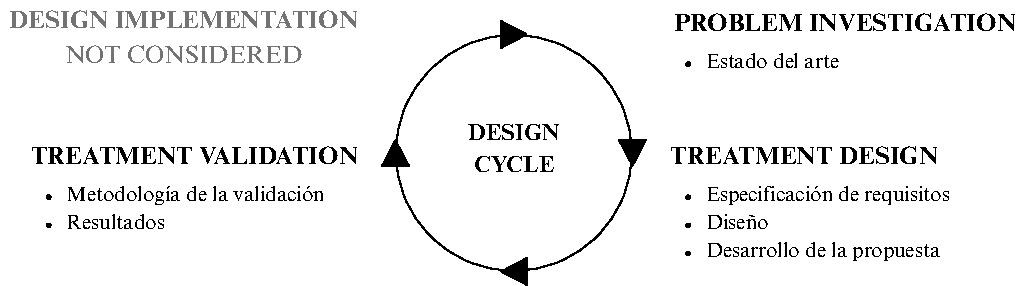
\includegraphics[width=0.9\textwidth]{tfgetsinf/images/Design cycle.pdf}
\caption{Ciclo de Diseño.}
\label{fig:ciclo_diseno}
\end{figure}

El ciclo de diseño se compone de tres fases principales: la investigación del problema, el diseño del tratamiento y la validación del tratamiento. Este conjunto de actividades se denomina ciclo de diseño porque los investigadores suelen iterar repetidamente sobre estas fases a lo largo de un proyecto de investigación basado en \textit{Design Science}.  A continuación, se explican las tres fases:
\begin{enumerate}
    \item Investigación del problema (\textit{Problem Investigation}): Se analiza en profundidad el contexto y los elementos clave del problema que se quiere abordar. En esta fase se identifican los \textit{stakeholders} y se definen los objetivos, así como los efectos y consecuencias que puede tener el desarrollo respecto a dichos objetivos. Además, se lleva a cabo un análisis del estado del arte, evaluando soluciones existentes y enfoques previos, lo que permite comprender mejor las limitaciones actuales y justificar la necesidad de una nueva propuesta.
    
    \item Diseño de la solución (\textit{Treatment Design}): En esta fase se genera la solución para dar respuesta a las limitaciones identificadas en la etapa anterior. Para ello, se lleva a cabo un proceso que abarca el diseño e implementación de la solución.
     
    \item Validación de la solución (\textit{Treatment Validation}): Se comprueba que la implementación del artefacto ha cumplido con los objetivos iniciales en la práctica. Algunas de las preguntas ligadas a esta fase se plantean el efecto real del tratamiento, la aceptación por parte de los usuarios y su eficacia. En definitiva, la validación permite detectar posibles limitaciones o áreas de mejora, lo que puede dar lugar a nuevas iteraciones sobre el diseño de la solución. 
\end{enumerate}

\subsection{Preguntas de investigación}
Para guiar el trabajo dentro de cada una de estas fases, se ha formulado una serie de preguntas de investigación. Estas preguntas están diseñadas para orientar el proceso de desarrollo, desglosar el problema y asegurar que la solución propuesta responde a las necesidades identificadas. 
Las preguntas han sido clasificadas en función de cada una de las fases metodológicas.

\textbf{Fase 1: Investigación del problema}
\begin{enumerate}
    \item ¿Cuál es la base de genética que sustentan los análisis PRS? 
    \item ¿Qué herramientas tecnológicas dan soporte a la ejecución de análisis PRS? 
    \item ¿Cuáles son las principales barreras y limitaciones que enfrentan los usuarios de estas herramientas tecnológicas? 
\end{enumerate}

\textbf{Fase 2: Diseño de la solución}
\begin{enumerate}
    \item ¿Qué requisitos debe cumplir una plataforma web para superar las barreras identificadas y facilitar el análisis PRS? 
    \item ¿Cuál es la arquitectura tecnológica más adecuada para esta plataforma? 
    \item ¿Cómo optimizar la carga, procesamiento y análisis de modelos PRS?     
\end{enumerate}

\textbf{Fase 3: Validación de la solución}
\begin{enumerate}
    \item ¿En qué medida la plataforma desarrollada cumple con los requisitos establecidos para superar las barreras identificadas en el análisis PRS?
    \item ¿Cuál es el nivel de usabilidad y utilidad percibida por los usuarios finales al interactuar con la plataforma?
\end{enumerate}

\subsection{\textit{Stakeholders}}
En este apartado se busca identificar los distintos grupos de interés del proyecto o \textit{stakeholders}. Según la metodología \textit{design science} (explicada en la sección~\ref{section:metodologia}), un \textit{stakeholder} es una persona, grupo de personas o institución que se ve afectada por el tratamiento de un problema. Identificarlos correctamente es fundamental, ya que de ellos surgen tanto los objetivos como las restricciones del proyecto que, a su vez, son la base para definir los requisitos que debe cumplir la solución desarrollada. 

Depende del tipo de problema, puede que los \textit{stakeholders} no sepan que lo son aún, por ejemplo, en los proyectos exploratorios, ya que los objetivos no están bien definidos al inicio de estos. En cambio, como en el caso de este proyecto, en los guiados por la utilidad, existen partes interesadas con objetivos definidos a los que la investigación debe contribuir. 

Se pueden encontrar diferentes tipos de \textit{stakeholders}; siendo identificados en este trabajo los siguientes para este proyecto: 
\begin{itemize}
    \item Investigadores en el ámbito de la genómica, más concretamente en análisis PRS. Serían los principales beneficiarios del desarrollo de esta plataforma, ya que son los que tienen unos objetivos claros acerca de la expectativa del resultado.
    \item Profesionales sanitarios como genetistas clínicos y asesores genéticos. A través de esta herramienta, podrían integrar los análisis PRS en su práctica clínica, gracias a que la plataforma ha sido diseñada para facilitar su uso por parte de profesionales sin conocimientos técnicos avanzados previos.
    \item Pacientes, quienes, aun sin interactuar directamente con la plataforma, se benefician de su uso por parte de profesionales clínicos, mejorando la prevención de enfermedades y diagnósticos. Su atención clínica en general se ve favorecida.
    \item Entidades colaboradoras, como centros de investigación, universidades, hospitales o biobancos, que podrían incorporar esta solución como parte de su infraestructura tecnológica.
\end{itemize}
De forma directa o indirecta, este grupo de personas o entidades se podría ver beneficiado por el desarrollo de la plataforma \textit{Phenoscore}.

\subsection{Aplicación de la metodología}
La aplicación de la metodología \textit{Design Science} se plasma en la organización del documento: cada fase metodológica encuentra su correspondencia en uno o varios capítulos, de modo que las cuestiones planteadas se van resolviendo de forma progresiva y coherente a lo largo de la memoria.

La primera fase, llamada investigación del problema, se ha resuelto en el Capítulo ~\ref{chap:investigación} (\nameref{chap:investigación}).

\begin{itemize}
    \item \textbf{Capítulo ~\ref{chap:introducción}. \nameref{chap:introducción}}: Se encarga de introducir y contextualizar el problema.También se presenta la motivación del proyecto, sus objetivos, la metodología empleada y los \textit{stakeholders} identificados.
    \item \textbf{Capítulo ~\ref{chap:investigación}. \nameref{chap:investigación}}: En este capítulo se da respuesta a las preguntas de investigación de dicha fase, analizando los fundamentos de los análisis PRS y se analizan los artefactos existentes que han dado algún tipo de solución a la ejecución de análisis PRS o a alguna fase de su configuración y se comparan esas soluciones con la propuesta presentada.
\end{itemize}

La segunda fase, llamada diseño de la solución, se ha resuelto en el capítulo ~\ref{chap:diseño} (\nameref{chap:diseño}).

\begin{itemize}
    \item \textbf{Capítulo ~\ref{chap:diseño}. \nameref{chap:diseño}}: en la sección ~\ref{section:especificación} se han detectado las oportunidades de mejora y se han definido las características y funcionalidades necesarias para el desarrollo a través de los requisitos como: historias de usuario, requisitos funcionales y no funcionales. Posteriormente, se ha realizado el modelado conceptual junto con las posibles soluciones identificadas y la solución propuesta.
    
    Por lo que se refiere a la tecnología y el diseño de la interfaz, ambas cuestiones se han resuelto en la sección ~\ref{section:diseño}; se han descrito las herramientas que se van a usar junto con la estructura de la solución. Además, a través de los \textit{mockups} se ha representado la idea del diseño visual de la aplicación.

    Por otro lado, en la sección ~\ref{section:desarrollo} se ha llevado a cabo la implementación de las funcionalidades anteriormente identificadas en el análisis.
    
\end{itemize}

La última fase, llamada validación de la solución, se ha resuelto en el capítulo ~\ref{chap:pruebas} (\nameref{chap:pruebas}).

\begin{itemize}
    \item \textbf{Capítulo ~\ref{chap:pruebas}. \nameref{chap:pruebas}}: se detalla la metodología de validación, los participantes, el procedimiento seguido y los instrumentos de medición empleados. Se presentan los resultados, incluyendo la validación funcional, la evaluación de requisitos no funcionales, la aceptación tecnológica y la matriz de trazabilidad. Además, se analiza si la solución ha resultado satisfactoria respecto a las expectativas y necesidades de los \textit{stakeholders}.
\end{itemize}

Por último, se han presentado las conclusiones del trabajo en el capítulo ~\ref{chap:conclusiones} 
(\nameref{chap:conclusiones}).

\begin{itemize}
    \item \textbf{Capítulo ~\ref{chap:conclusiones}. \nameref{chap:conclusiones}}: se sintetizan los resultados del trabajo, se establecen relaciones con las competencias del grado y se señalan posibles mejoras y líneas de evolución futura.
\end{itemize}

%%%%%%%%%%%%%%%%%%%%%%%%%%%%%%%%%%%%%%%%%%%%%%%%%%%%%%%%%%%%%%%%%%%%%%%%%%%%%%%
%                         CAPITOLS (tants com calga)                          %
%%%%%%%%%%%%%%%%%%%%%%%%%%%%%%%%%%%%%%%%%%%%%%%%%%%%%%%%%%%%%%%%%%%%%%%%%%%%%%%

\chapter{Investigación del problema}
\label{chap:investigación}

\section{Fundamentos de las puntuaciones de riesgo poligénico}

Las Puntuaciones de Riesgo Poligénico (PRS) son una métrica que cuantifica la predisposición genética de un individuo a un rasgo o enfermedad, basándose en la suma de los efectos de múltiples variantes genéticas. Para comprender su construcción y aplicación, es fundamental entender los conceptos genéticos y estadísticos en los que se basan. Esta sección da respuesta a la primera pregunta de investigación: ¿Cuál es la base de genética que sustentan los análisis PRS?

El material de partida para cualquier PRS son los resultados de los Estudios de Asociación del Genoma Completo (GWAS, del inglés \textit{Genome Wide Association Study}) \cite{babb, uffelmann}. Estos estudios a gran escala analizan los genomas de miles de individuos para identificar Polimorfismos de un Solo Nucleótido (SNPs, del inglés \textit{Single Nucleotide Polymorphism}) \cite{choi} que están estadísticamente asociados con una enfermedad. Para cada SNP que supera un umbral de significancia estadística, el GWAS proporciona un tamaño del efecto ($\beta_j$), que refleja la magnitud de su asociación con la patología. Estos tamaños de efecto se convierten en los pesos que se utilizarán como parámetros en el modelo PRS.

La construcción de un modelo PRS a partir de los datos brutos de un GWAS es un proceso bioinformático complejo que va más allá de una simple suma. Antes de aplicar la fórmula, se deben realizar varios pasos metodológicos cruciales para asegurar la validez del modelo, como la selección de SNPs mediante un umbral de p-valor (\textit{p-value thresholding}) y la poda de variantes en desequilibrio de ligamiento (\textit{LD clumping}). 

Este último paso es esencial, ya que el desequilibrio de ligamiento se refiere al fenómeno por el cual variantes genéticas que están físicamente cercanas en un cromosoma tienden a heredarse juntas. La poda, por tanto, elimina las variantes redundantes, asegurando que los SNPs incluidos en el modelo sean en gran medida independientes entre sí y evitando así una sobreestimación del riesgo \cite{lambert2019}.

Una vez se dispone del conjunto final de SNPs y sus pesos, la puntuación para un individuo $i$ se calcula mediante un modelo de regresión lineal aditivo:
$$PRS_i = \sum_{j=1}^{n}  G_{ij} \, \beta_j$$ donde $\beta_j$ representa el efecto de cada variante, $G_{ij}$ el número de copias de la variante que posee el individuo \footnote{El valor puede ser 0, 1 o 2. Esto se debe a que los seres humanos heredan dos copias de cada cromosoma, una de cada progenitor. Así, para un SNP concreto, un individuo puede no haber heredado ninguna copia del alelo de riesgo, haber heredado una o haber heredado ambas.}, y $n$ el número total de variantes asociadas \cite{choi, collister}. Al aplicar este modelo al genoma de un individuo, se obtiene un valor numérico que estima su predisposición genética.

El valor bruto de un PRS no es directamente interpretable. Para obtener un significado clínico, debe ser contextualizado comparándolo con las puntuaciones de una gran población de referencia, lo que permite situar al individuo en un percentil de riesgo relativo (ej. ''en el 5\% superior de riesgo genético'') \cite{maamari, corpas}.

La principal utilidad clínica del PRS es la estratificación del riesgo para la medicina preventiva. Un ejemplo de alto impacto es en las enfermedades cardiovasculares. Un individuo puede tener factores de riesgo tradicionales (colesterol, presión arterial) en un rango intermedio, pero un PRS elevado puede reclasificarlo a una categoría de alto riesgo, justificando el inicio de un tratamiento preventivo (como estatinas) mucho antes de lo que se haría de otra manera \cite{knowles}. De este modo, el PRS no reemplaza los factores de riesgo clásicos, sino que los complementa, añadiendo una nueva capa de información para una toma de decisiones más precisa \cite{terkelsen}.

A pesar de su gran potencial, la implementación clínica de los PRS enfrenta desafíos significativos. Uno de los más importantes es la portabilidad entre diferentes poblaciones ancestrales. La gran mayoría de los GWAS se han realizado en individuos de ascendencia europea, lo que significa que los modelos PRS derivados de ellos son significativamente menos precisos cuando se aplican a individuos de ascendencia africana, asiática u otras. Esta falta de diversidad en los datos de entrenamiento es una barrera crítica para una implementación equitativa de la genómica en la salud \cite{torkamani2018}.

Además, la comunicación de un riesgo probabilístico y genético a los pacientes es un desafío en sí mismo, requiriendo un asesoramiento genético cuidadoso para evitar el determinismo genético y la ansiedad innecesaria \cite{alliance}. 

En conclusión, los análisis de PRS representan un avance fundamental en la medicina genómica. Aunque su implementación a gran escala aún enfrenta retos metodológicos y éticos, su potencial para guiar intervenciones preventivas y personalizar el tratamiento es innegable, marcando el camino hacia una práctica clínica más proactiva y precisa \cite{wray}.


\section{Estado del arte}
Como se ha mencionado en la introducción, los \textit{Polygenic Risk Scores} (PRS) se han convertido en una herramienta prometedora en la medicina de precisión al permitir estimar el riesgo genético de un individuo para desarrollar enfermedades complejas. Los PRS representan un avance significativo respecto a los enfoques tradicionales que se centraban en el estudio de enfermedades simples, donde la causa de la enfermedad radica en una única variante.

Para realizar un análisis de PRS se requiere un modelo PRS para la enfermedad de estudio y los datos genómicos del individuo de interés. Hay múltiples pasos involucrados en el proceso completo, algunos de esos pasos y las herramientas que se usan en ellos se pueden observar en la siguiente tabla:

\begin{table}[H]
    \centering
    \small
    \begin{tabularx}{\textwidth}{ >{\raggedright\arraybackslash}X >{\raggedright\arraybackslash}X >{\raggedright\arraybackslash}X }
        \toprule
        \textbf{Paso del Proceso} & \textbf{Herramienta(s) Utilizada(s)} & \textbf{Referencias} \\
        \midrule
        Control de calidad de los \textit{datasets} y variaciones & 
        • \texttt{PLINK} (es el estándar para el filtrado estadístico). \newline 
        • \texttt{BCFtools} (muy potente para la manipulación y filtrado de ficheros \textit{VCF}). 
        & \texttt{PLINK} \textit{QC Manual}, \texttt{BCFtools} \textit{Documentation}
        \\ \addlinespace

        Alineamiento entre datos del paciente y del modelo & 
        \texttt{PLINK} (se usa para armonizar los \textit{datasets}, asegurando que las variantes coincidan). 
        & \texttt{PLINK} \textit{PCA Tutorial}
        \\ \addlinespace

        Estimación y ajuste de ancestría del paciente & 
        \texttt{PLINK} (se utiliza para realizar el Análisis de Componentes Principales o PCA). 
        & \textit{AncestryCheck} with \texttt{plinkQC}
        \\ \addlinespace

        Preparación de la población de referencia &  
        • \texttt{PLINK} y \texttt{BCFtools} (para el control de calidad). \newline 
        • \texttt{bgenix} (para indexar y acceder a datos masivos). 
        & \textit{BGEN Documentation}, \textit{BGENIX Documentation}
        \\ \addlinespace

        Creación del Modelo PRS y Cálculo de la Puntuación & 
        • \texttt{PRSice2} (implementa el método de ''\textit{Clumping + Thresholding}''). \newline 
        • \texttt{LDpred2} (implementa un método Bayesiano más avanzado). 
        & \texttt{PRSice-2}: \textit{Polygenic Risk Score software}, \texttt{LDpred2}: \textit{better, faster, stronger}
        \\
        \bottomrule
    \end{tabularx}
    \caption{Pasos, herramientas y referencias en el análisis PRS.}
    \label{tab:prs_workflow}
\end{table}

Como resultado, para poder ejecutar un análisis de PRS se deben combinar múltiples herramientas informáticas.

Es por ello que la aplicación de análisis PRS en entornos clínicos se enfrenta a una barrera fundamental: la alta complejidad y fragmentación del proceso. Como se ha mencionado, un análisis completo requiere una secuencia de pasos bien definidos y cada una de estas tareas suele ser ejecutada por herramientas informáticas especializadas y potentes, como \texttt{PLINK} o \texttt{BCFtools}. 

El primer problema radica en que la integración y orquestación manual de estas herramientas exige un conocimiento técnico avanzado en bioinformática, creando un flujo de trabajo fragmentado que resulta inaccesible para la mayoría de los investigadores clínicos. Debido a esta limitación, el paso lógico es buscar soluciones que ya integren estos pasos en un único \textit{pipeline} automatizado. 

Sin embargo, esto lleva a un segundo problema: la mayoría de estas soluciones carecen de una interfaz de usuario (\textit{UI}) intuitiva y funcionan a través de la línea de comandos. Esta es la complejidad que este trabajo pretende simplificar: no solo integrar el flujo de trabajo, sino también presentarlo a través de una interfaz accesible que elimine la barrera tecnológica para el usuario final.

Dado que el objetivo de este trabajo es facilitar la ejecución de análisis PRS para usuarios no expertos, se han investigado herramientas que integran \textit{software} existentes y automatizan muchos de los complejos pasos y decisiones de análisis.
Las principales herramientas para ejecutar análisis de PRS son las siguientes:

\begin{itemize}
   \item
    \texttt{pgsc\_calc} (\textit{Polygenic Score Catalog Calculator}) \cite{lambert2024}: se trata de un \textit{pipeline} \texttt{Nextflow} oficial del repositorio \textit{PGS Catalog}, diseñado exclusivamente para realizar análisis de PRS usando modelos existentes en el repositorio, o personalizados. Automatiza el proceso de descargar modelos de \textit{PGS Catalog} y aplicarlos a datos genéticos, en formato \textit{VCF}, \texttt{PLINK1} o \texttt{PLINK2}. \footnote{\textit{VCF (Variant Call Format)} es un formato de texto estándar para almacenar variaciones genéticas. \texttt{PLINK1} y \texttt{PLINK2} son los formatos nativos del \textit{software} \texttt{PLINK}, que utilizan un conjunto de archivos binarios (\texttt{.bed}, \texttt{.bim}, \texttt{.fam}) para una gestión eficiente de grandes \textit{datasets} genómicos.}. Genera como resultado un reporte resumen con los resultados del análisis, detalles del modelo aplicado y parámetros relevantes del proceso. 
    %El problema con este pipeline es su complejidad, además no tiene interfaz gráfica, se opera por consola y el reporte resultante es estático.
    
    \item
    \texttt{GenoPred} \textit{pipeline} \cite{pain2024}: se trata de un \textit{pipeline} escalable de \texttt{Snakemake} para generar y aplicar modelos PRS sobre datos genómicos, en varios formatos: \texttt{PLINK1}, \texttt{PLINK2}, \textit{VCF}, \textit{BGEN}, y \textit{23andMe}. Al igual que \texttt{pgsc\_calc}, permite realizar los análisis de PRS a partir de modelos PRS existentes, procedentes de repositorios de modelos como \textit{PGS Catalog} u otros. Sin embargo, además permite crear modelos PRS para seguidamente aplicarlos, ya que la herramienta ha sido desarrollada para facilitar la generación de modelos PRS empleando distintos \textit{softwares}. La salida principal de esta herramienta son archivos \textit{HTML} con resultados de análisis PRS y reportes técnicos. Además de la obtención del reporte de análisis, permite obtener cáculos intermedios de interés, como control de calidad o estimación de ancestrías de los datos de entrada.
    %%Sin embargo, es una herramienta  compleja ya que no dispone de interfaz y su uso es por línea de comandos. La instalación y uso de snakemake o conda puede ser un reto para los usuarios no expertos. 
     
    \item
     \texttt{PGS Calculator} (\texttt{pgs-calc} de Lukasz) \cite{lukfor_pgscalc}: es una herramienta de línea de comandos para aplicar modelos PRS a datos genómicos en formato \textit{VCF}. Se conecta a \textit{PGS Catalog} para descargar automáticamente los archivos de puntuación de los modelos o también permite cargar archivos de modelos PRS propios, pero no la creación de nuevos modelos. La salida es un \textit{HTML} interactivo con gráficos de distribución de PGS. 
     %Como en casos anteriores, no dispone de interfaz gráfica fuera del terminal y requiere línea de comandos. 

    \item
    \texttt{PRS Pipeline tutorial} (Collister \& Liu) \cite{collister}: es un tutorial práctico que permite aplicar un modelo PRS existente a datos genómicos del repositorio \textit{UK Biobank}. No es exactamente una herramienta integrada, pero ilustra todo el flujo desde la extracción de SNPs hasta el cálculo de PRS siguiendo un ejemplo concreto. 
    %Su mayor limitación es que no permite la ejecucuión de un análisis para un único individuo, ya que está orientada a los datos de UK Biobank.
    
\end{itemize}

\section{Principales barreras y limitaciones}

La mayor utilidad de estas herramientas es que integran todos los pasos necesarios para ejecutar un análisis PRS completo. Sin embargo, su principal limitación es que no disponen de una interfaz que permita configurar fácilmente los análisis de PRS. El uso por línea de comandos, así como la instalación y el uso de herramientas de orquestación de \textit{workflows} (\texttt{snakemake} o \texttt{nextflow}) y gestores de entornos de ejecución virtuales (\texttt{conda}), supone un reto para los usuarios no expertos.  Adicionalmente, el ``\texttt{PRS Pipeline tutorial}'' tiene la limitación específica de no ser apto para análisis de individuos únicos, ya que está orientado a conjuntos de datos a gran escala como los de \textit{UK Biobank}. 

\begin{table}[H]
    \centering
    \small
    \label{tab:prs_tool_limitations}
    \begin{tabularx}{\textwidth}{ >{\raggedright\arraybackslash}X >{\centering\arraybackslash}X >{\centering\arraybackslash}X >{\centering\arraybackslash}X >{\centering\arraybackslash}X }
        \toprule
        \textbf{Herramienta} & \textbf{Falta de Interfaz Gráfica (\textit{CLI})} & \textbf{Requiere Conocimiento Técnico Avanzado} & \textbf{Solo Aplica Modelos Existentes (No Creación)} & \textbf{No Apto para Análisis Individual} \\
        \midrule
        \texttt{pgsc\_calc} & Sí & Sí (\texttt{Nextflow}) & Sí & No \\ \addlinespace
        \texttt{GenoPred} \textit{pipeline} & Sí & Sí (\texttt{Snakemake}, \texttt{Conda}) & No & No \\ \addlinespace
        \texttt{PGS Calculator} & Sí & Sí (\textit{CLI}) & Sí & No \\ \addlinespace
        \texttt{PRS Pipeline tutorial} & Sí & Sí (Tutorial práctico) & Sí & Sí \\
        \bottomrule
    \end{tabularx}
    \caption{Limitaciones clave de las herramientas para análisis de PRS.}
\end{table}

El análisis PRS para predecir la predisposición genética a enfermedades complejas se ve significativamente limitado por su inherente complejidad técnica. El proceso, que abarca desde la descarga y preprocesamiento de datos genéticos hasta la ejecución de flujos de trabajo específicos para el cálculo y la interpretación de resultados, requiere un dominio avanzado de herramientas bioinformáticas y conocimientos especializados. Estas barreras técnicas restringen considerablemente el acceso y la adopción de los PRS por parte de investigadores con menor experiencia en bioinformática y profesionales del ámbito clínico.

A partir del estudio del estado del arte, se han identificado problemas recurrentes en las soluciones actuales: una elevada complejidad que dificulta el acceso y aprovechamiento, una fragmentación de funcionalidades que obliga al uso de múltiples plataformas, y la entrega de resultados en formatos planos que carecen de visualizaciones intuitivas para una rápida interpretación. Estos desafíos recalcan la necesidad de una innovación que centralice el proceso en una única herramienta, ofreciendo una experiencia más amigable y accesible que integre todas las fases del análisis PRS, desde la carga de datos genéticos hasta la interpretación visual de los resultados.
\input{capitulos/3-Diseño de la solución/cap3_diseño_de_la_solución}
\input{capitulos/4-Validación de la solución/cap4_validación_de_la_solución}

%%%%%%%%%%%%%%%%%%%%%%%%%%%%%%%%%%%%%%%%%%%%%%%%%%%%%%%%%%%%%%%%%%%%%%%%%%%%%%%
%                                 CONCLUSIONS                                 %
%%%%%%%%%%%%%%%%%%%%%%%%%%%%%%%%%%%%%%%%%%%%%%%%%%%%%%%%%%%%%%%%%%%%%%%%%%%%%%%

\chapter{Conclusiones}
\label{chap:conclusiones}

Este capítulo final permite realizar una síntesis de los objetivos obtenidos, el logro de los objetivos, la reflexión sobre los desafíos durante el proceso y los esfuerzos de aprendizaje. El propósito es presentar resultados y reflexiones de manera clara y crítica para este trabajo final.

\section{Respuesta a las Preguntas de Investigación}

Este capítulo final presenta una síntesis del trabajo realizado, evaluando los hallazgos del proyecto a través de las preguntas de investigación planteadas en la metodología. El propósito es demostrar de manera clara y crítica cómo el proceso de diseño, desarrollo y validación ha dado respuesta a cada una de estas cuestiones.

\subsection{Fase 1: Investigación del Problema}

La primera fase del proyecto buscaba establecer las bases teóricas y contextuales. Las preguntas de investigación asociadas eran:

\begin{itemize}
    \item \textit{¿Cuál es la base de genética que sustentan los análisis PRS?}
    \item \textit{¿Qué herramientas tecnológicas dan soporte a la ejecución de análisis PRS?}
    \item \textit{¿Cuáles son las principales barreras y limitaciones que enfrentan los usuarios de estas herramientas tecnológicas?}
\end{itemize}

El Capítulo 2 ha respondido a estas preguntas de forma exhaustiva. Se ha determinado que los análisis PRS se fundamentan en los resultados de los estudios \textit{GWAS}, que identifican variantes genéticas (SNPs) asociadas a enfermedades y cuantifican su efecto. El análisis del estado del arte reveló que, si bien existen herramientas potentes como \textit{pgs\_calc} o \textit{GenoPred}, su principal barrera es la alta complejidad técnica, su dependencia de la línea de comandos (\textit{CLI}) y la fragmentación del flujo de trabajo. Esta investigación confirmó la necesidad de una solución integrada y usable para usuarios no expertos en bioinformática.

\subsection{Fase 2: Diseño de la Solución}

La segunda fase se centró en definir la solución técnica. Las preguntas de investigación eran:

\begin{itemize}
    \item \textit{¿Qué requisitos debe cumplir una plataforma web para superar las barreras identificadas y facilitar el análisis PRS?}
    \item \textit{¿Cuál es la arquitectura tecnológica más adecuada para esta plataforma?}
    \item \textit{¿Cómo optimizar la carga, procesamiento y análisis de modelos PRS?}
\end{itemize}

El Capítulo 3 da respuesta a estas cuestiones a través del diseño de \textit{PhenoScore}. Se definieron requisitos funcionales centrados en la usabilidad y la abstracción de la complejidad (ej. HU05: Subida de archivos mediante una interfaz gráfica). Se diseñó una arquitectura por capas (Presentación, Lógica de Negocio, Datos) para garantizar la mantenibilidad y escalabilidad. Para optimizar la carga de los análisis, se propuso una arquitectura asíncrona basada en una cola de trabajos, que permite ejecutar procesos computacionalmente intensivos en segundo plano sin bloquear la interfaz de usuario, respondiendo así al reto del rendimiento.

\subsection{Fase 3: Validación de la Solución}

La fase final buscaba evaluar la idoneidad y el éxito de la plataforma implementada. Las preguntas de investigación eran:

\begin{itemize}
    \item \textit{¿En qué medida la plataforma desarrollada cumple con los requisitos establecidos para superar las barreras identificadas?}
    \item \textit{¿Cuál es el nivel de usabilidad y utilidad percibida por los usuarios finales al interactuar con la plataforma?}
\end{itemize}

El Capítulo 4 responde a estas preguntas a través de un meticuloso proceso de validación. Los resultados demuestran que \textit{PhenoScore} cumple plenamente con los requisitos funcionales, ya que el 100\% de los usuarios completó con éxito todas las tareas clave. El nivel de usabilidad y utilidad percibida, medido tanto cualitativamente (tiempos de tarea) como cuantitativamente (Modelo de Aceptación Tecnológica), fue muy alto. Es especialmente relevante que el perfil de usuario no técnico pudiera utilizar la herramienta de forma autónoma, lo que confirma que la plataforma supera con éxito la barrera de accesibilidad que motivó el proyecto. La alta puntuación en las escalas de Facilidad de Uso y Utilidad Percibida del \textit{TAM} refuerza esta conclusión.

\section{Desafíos y soluciones del desarrollo}
Durante la fase de implementación, surgieron varios desafíos técnicos, algunos de los cuales tuvieron que ser superados con un análisis y toma de decisiones sustanciales para garantizar el éxito del proyecto.

\begin{itemize}
    \item \textbf{Problema de Entorno y Compatibilidad:} El obstáculo más significativo fue la inestabilidad encontrada al intentar ejecutar el \textit{pipeline} de \textit{GenoPred} en el Subsistema de \textit{Windows} para \textit{Linux (WSL)}. Se lanzó una actualización de la herramienta externa introdujo cambios que rompían la compatibilidad y causaban errores fatales.
    \newline
    \textbf{Solución:} La arquitectura de despliegue completa se migró a una máquina virtual ejecutada en \textit{Google Cloud Platform} con un sistema operativo \textit{Linux} nativo. Fue un gran esfuerzo de reconfiguración, pero se logró un entorno de ejecución sólido, predecible y escalable, que es fundamental para una aplicación de estas características.
    
    \item \textbf{Dependencia de Software Externo:} Tras la migración, los análisis seguían fallando debido a un \textit{bug} introducido en la nueva versión de \textit{GenoPred}. La depuración de este problema fue compleja, ya que la causa se encontraba en código de terceros.
        \newline
        \textbf{Solución:} Resolver este problema fue posible después de una investigación proactiva que incluyó el análisis de \textit{logs}, la revisión de la documentación y, finalmente, el contacto directo con el desarrollador principal de la herramienta. Su colaboración fue clave para identificar y corregir el \textit{bug}, lo que permitió desbloquear el desarrollo. En general, fue un buen ejemplo de comunicación en proyectos que dependen en gran medida del software de código abierto.
        
    \item \textbf{Limitación de la Concurrencia:} Durante la validación, se identificó que la herramienta subyacente, \textit{Snakemake}, no permite ejecuciones concurrentes en el mismo directorio de proyecto \cite{snakemake}.
        \newline
        \textbf{Solución (Conceptual):} Aunque no se implementó por estar fuera del alcance del TFG, se identificó la solución técnica necesaria: aislar la ejecución de cada trabajo, por ejemplo, creando una copia dinámica actualizada del proyecto para cada análisis. Este análisis demuestra una comprensión del problema y establece una línea clara para trabajo futuro.
    
\end{itemize}

En cuanto a los errores cometidos, una posible mejora habría sido realizar un análisis técnico más detallado de las dependencias externas (\textit{GenoPred/Snakemake}) en una fase más temprana del diseño. Una prueba de concepto inicial sobre la concurrencia probablemente haber revelado la limitación de \textit{Snakemake} antes, lo que habría permitido preparar una solución a tiempo.

\section{Aprendizaje}

La realización de este Trabajo de Fin de Grado ha aportado una valiosa oportunidad de aprendizaje, tanto desde el punto de vista técnico como personal. 

En términos profesionales, el proyecto brinda la oportunidad de aplicar y profundizar en una amplia variedad de competencias relacionadas con la ingeniería del software. Uno de los aspectos más destacados ha sido el diseño de una arquitectura de software compleja y moderna, que implica la implementación de un sistema asíncrono basado en colas de mensajes, un desafío técnico mucho mayor en comparación con una aplicación web común. La necesidad de integrar y depurar herramientas bioinformáticas existentes ha proporcionado una valiosa experiencia en la adopción e identificación de dependencias y resolución de problemas en un entorno real.

Como conclusión personal, creo que el aprendizaje más significativo ha sido la gestión de la incertidumbre y la resiliencia. Lidiar con dificultades paralizantes de las que yo no era responsable directa, como el \textit{bug} en \textit{GenoPred}, me ha enseñado la importancia de la paciencia, la investigación minuciosa y la comunicación persistente para resolver los problemas. Este proyecto me ha dado la capacidad para tomar decisiones técnicas y gestionar un proyecto completo de software.

\section{Trabajo a futuro}
El estado actual de \textit{PhenoScore} representa una base sólida y funcional, pero también un punto de partida con un gran espacio para el desarrollo. Las siguientes líneas de trabajo futuro podrían llevar a la evolución de la plataforma a una solución más sólida y completa y estar lista para un uso a mayor escala.

\subsubsection{Despliegue y pruebas de rendimiento en un entorno de producción}
El siguiente paso más importante consiste en el despliegue de la aplicación en un entorno de producción accesible públicamente. Esto  permite realizar pruebas reales de rendimiento de la aplicación y, a su vez, terminar con la validación de todos los requisitos no funcionales. Una vez desplegada, se podría ejecutar la auditoría de \textit{Google Lighthouse} para obtener métricas en aspectos como rendimiento, accesibilidad, buenas prácticas, o también pruebas de carga para evaluar cómo responde el sistema ante la concurrencia de varios usuarios.

\subsubsection{Implementación de una solución para la ejecución concurrente}
Durante la validación se ha constatado que la limitación principal de la parte de análisis es no poder ejecutarlos de forma concurrente debido a las limitaciones de \textit{Snakemake}. La siguiente fase de trabajo tendría que centrarse en solucionar este problema. La forma más viable sería el aislamiento completo del entorno de ejecución de cada trabajo. Así, al comenzar un nuevo análisis, el \textit{worker} no sólo generaría los ficheros de configuración, sino que haría también una copia propia y aislada del \textit{pipeline} de \textit{GenoPred} en un directorio temporal. De esta manera, la cola de trabajos podría tener en paralelo muchos análisis en paralelo y se podría mejorar mucho la velocidad y la escalabilidad del sistema.

\subsubsection{Gestión centralizada de pacientes y poblaciones de referencia}
Actualmente, la plataforma requiere que el usuario suba los datos genómicos del paciente cada vez que se crea un nuevo análisis. Para mejorar la eficiencia y la usabilidad, una línea de trabajo futuro clave es la creación de un módulo de gestión de pacientes. Esto permitiría a los usuarios almacenar de forma segura y centralizada la información de sus cohortes de pacientes, pudiendo seleccionar un paciente existente al crear un nuevo análisis en lugar de subir sus datos repetidamente.

Del mismo modo, se podría desarrollar una funcionalidad para que usuarios o administradores suban y gestionen poblaciones de referencia personalizadas. De momento no se ha podido desarrollar esta tarea por no disponer del suficiente recurso computacional para almacenar y procesar estos enormes conjuntos de datos. Habilitar esta opción permitiría a los investigadores usar sus propias cohortes de referencia y ser más versátiles y precisas sus ejecuciones de los análisis.

\subsubsection{Creación de documentación y tutoriales para usuarios}
Para facilitar la adopción de la plataforma por parte de nuevos usuarios, es fundamental desarrollar una sección de documentación y tutoriales interactivos. Esta sección podría incluir:
\begin{itemize}
\item Un manual de usuario que explique detalladamente cada funcionalidad de la plataforma.
\item Videotutoriales que guíen a los usuarios a través del proceso completo de creación y ejecución de un análisis.
\item Una sección de Preguntas Frecuentes (FAQ) para resolver las dudas más comunes.
\end{itemize}
Una buena documentación es necesaria para asegurar que los usuarios, especialmente los no técnicos, puedan sacar el máximo provecho de la herramienta de forma autónoma.

\subsubsection{Pruebas de Concurrencia y Escalabilidad a Gran Escala}
Uno de los mayores potenciales de mejora para \textit{PhenoScore} es la implementación de la ejecución concurrente de análisis. Durante el desarrollo, se identificó que la herramienta externa \textit{Snakemake} presenta una limitación que impide ejecuciones paralelas en el mismo directorio.

La siguiente fase de trabajo debería centrarse en implementar la solución de aislamiento de directorios ya diseñada conceptualmente. Al hacer que el \textit{worker} cree una copia temporal y aislada del \textit{pipeline} para cada trabajo, la cola podría procesar múltiples análisis en paralelo. Esta mejora transformaría el rendimiento \textit{throughput} del sistema, siendo un paso indispensable para su escalabilidad y su uso en entornos con múltiples usuarios.


\section{Relación del trabajo con los estudios cursados}

El desarrollo del presente TFG ha supuesto la materialización práctica de la transversalidad de las competencias adquiridas a lo largo del Grado en Ingeniería Informática, al no tratarse de un desarrollo aislado, sino de un sistema caracterizado por la multidisciplinariedad.

A continuación, se detalla la relación del trabajo con las principales áreas de conocimiento del grado.

\paragraph{Ingeniería del Software, Análisis de Requisitos y Validación}

En general, el proyecto se ha llevado a cabo siguiendo un proceso de ingeniería del software con un alto nivel de rigor a la hora de aplicar los fundamentos aprendidos en la especialización directamente al conjunto de fases, actividades y tareas realizadas. El uso de la metodología de la Ciencia del Diseño ha permitido una aplicación sistemática de las fases del ciclo de vida del software mencionadas anteriormente a lo largo de la etapa, que abarcan desde su concepción hasta la de los procesos que las finalizan, logrando una integración de las competencias de asignaturas como:

\begin{itemize}
\item La asignatura de Ingeniería del Software ha proporcionado la base metodológica para estructurar todo el proyecto. Conceptos como el ciclo de vida, la gestión de la configuración y la importancia de seguir un proceso definido han sido la estructura del trabajo, asegurando que cada fase (análisis, diseño, implementación, validación) se abordara de forma ordenada y coherente.

\item A partir de esta base, se han aplicado las técnicas de la asignatura Análisis y Especificación de Requisitos. Lo cual, se ha materializado en la obtención de las necesidades del usuario mediante historias de usuario y su posterior traducción a requisitos funcionales y no funcionales detallados. Asimismo, se ha realizado el modelado conceptual del sistema utilizando un conjunto completo de diagramas UML (Clases, Secuencia, Componentes, Despliegue), una competencia central en esta materia que ha sido clave para definir la estructura y el comportamiento de la solución antes de su implementación.

\item Finalmente, la asignatura Análisis, Validación y Depuración de Software ha guiado la última fase del proyecto. El capítulo de Validación se basa directamente en los principios para asegurar la calidad del producto. Se ha planificado y ejecutado un proceso de validación que incluye la verificación de la funcionalidad mediante un guion de tareas guiadas, la medición de requisitos no funcionales de rendimiento y la evaluación de la aceptación del usuario con el modelo TAM. Este enfoque demuestra la capacidad para diseñar y ejecutar un plan de pruebas que asegure que el software no solo funciona, sino que también cumple con los estándares de calidad definidos.

\end{itemize}

\paragraph{Diseño de Software.}
Uno de los pilares del TFG ha sido el diseño de una arquitectura de software moderna y compleja, un desafío central en la Ingeniería del Software. Se han aplicado directamente conceptos de la asignatura Diseño de Software, como la arquitectura por capas (Presentación, Lógica de Negocio y Persistencia) para garantizar la separación de responsabilidades y la mantenibilidad. 
Más allá de esta estructura, se han implementado varios patrones de diseño y buenas prácticas para resolver problemas específico, como: 

\begin{itemize}
    \item El patrón de cola de trabajos, para gestionar la ejecución de los análisis PRS: que son tareas de larga duración, se ha implementado este patrón utilizando \textit{BullMQ} y \textit{Redis}. Esto desacopla la petición del usuario de la ejecución real, evitando el bloqueo de la interfaz y mejorando la escalabilidad y la resiliencia del sistema.
    \item Principio de Responsabilidad Única: Este principio de diseño \textit{SOLID} \cite{martin} se ha aplicado al separar la lógica del \textit{AutoWorker} (cuya única responsabilidad es gestionar la cola) de la del \textit{AnalysisProcessor} (cuya única responsabilidad es ejecutar un análisis). Esta separación ha hecho el código mucho más limpio, mantenible y fácil de depurar.
\end{itemize}

\paragraph{Bases de Datos y Persistencia de la Información.}
Por otra parte, el proyecto ha requerido que se apliquen de manera directa y avanzada los conceptos de persistencia de datos, cuya formación básica ha sido la impartida en la asignatura de Bases de Datos y sistemas de información. En particular, la asignatura presentada anteriormente ha asentado las bases del conocimiento acerca del modelo relacional y de SQL, y ha permitido abordar con éxito el diseño e implementación de \textit{PhenoScore}.

\begin{itemize}
\item Diseño Relacional: El esquema de datos relacional, complejo, normalizado y optimizado para la plataforma ha sido diseñado e implementado en un servidor \textit{MariaDB}. Este proceso de modelado ha evolucionado desde un esquema de clases conceptual a un diagrama de entidad-relación físico y es una implementación directa de las habilidades de diseño de bases de datos.

\item Gestión y Consulta: Para la interacción con la base de datos, se ha utilizado un \textit{ORM} moderno como \textit{Prisma}. Aunque esta herramienta abstrae la escritura de SQL directo, la capacidad para construir consultas seguras y eficientes, así como para gestionar las migraciones del esquema, se fundamenta en la comprensión del modelo relacional y de cómo funcionan las operaciones subyacentes.

\item Bases de Datos \textit{NoSQL}: Adicionalmente, se ha utilizado una base de datos en memoria clave-valor como \textit{Redis} para una tarea de alta velocidad, en este caso, la gestión de la cola de trabajos. De esta manera uno puede ver cómo abordar más allá del modelo relacional y elegir la tecnología de persistencia más adecuada para cada requisito específico del sistema, un concepto avanzado en la gestión de la información.
\end{itemize}

\paragraph{Sistemas Operativos y Concurrencia.}
La funcionalidad central del proyecto, la ejecución asíncrona de análisis, es una aplicación directa de los conceptos fundamentales estudiados en asignaturas como Sistemas Operativos y Concurrencia. El conocimiento teórico adquirido con respecto de la gestión de procesos, su ciclo de vida y la comunicación entre los mismos, ha sido indispensable para poder diseñar la arquitectura del \textit{worker}.

Gracias a esta base conceptual, fue posible implementar la ejecución de \textit{GenoPred} como un proceso externo utilizando el módulo \textit{child\_process} de \textit{Node.js}, comprendiendo los mecanismos subyacentes de creación y monitorización de procesos que el sistema operativo gestiona.

En conclusión, este TFG es un reflejo de la formación recibida a lo largo del grado en un proyecto integrador en el que se han puesto en práctica las competencias adquiridas en las principales áreas de la informática de manera integrada para desarrollar una solución \textit{software} de un cierto nivel de complejidad.

%%%%%%%%%%%%%%%%%%%%%%%%%%%%%%%%%%%%%%%%%%%%%%%%%%%%%%%%%%%%%%%%%%%%%%%%%%%%%%%
%                                BIBLIOGRAFIA                                 %
%%%%%%%%%%%%%%%%%%%%%%%%%%%%%%%%%%%%%%%%%%%%%%%%%%%%%%%%%%%%%%%%%%%%%%%%%%%%%%%

\begin{thebibliography}{10}

    \bibitem{lander2001}
       Lander ES, Linton LM, Birren B, Nusbaum C, Zody MC, Baldwin J, et al.
       \newblock Initial sequencing and analysis of the human genome.
       \newblock Nature. 2001 Feb 15;409(6822):860-921.

    \bibitem{robinson}
       Robinson TR, Spock L.
       \newblock Genetics For Dummies.
       \newblock 3rd ed. Hoboken: Wiley; 2020.

    \bibitem{visscher}
       Visscher PM, Yengo L, Cox NJ, Wray NR.
       \newblock Discovery and implications of polygenicity of common diseases.
       \newblock Science. 2021 Sep 24;373(6562):1468-73. doi: 10.1126/science.abi8206.

    \bibitem{ye}
       Ye Y, Chen X, Han J, Jiang W, Natarajan P, Zhao H.
       \newblock Interactions between enhanced polygenic risk scores and lifestyle for cardiovascular disease, diabetes, and lipid levels.
       \newblock Circ Genom Precis Med. 2021 Feb;14(1):e003128. doi: 10.1161/CIRCGEN.120.003128.
    
    \bibitem{lewis}
       Lewis CM, Vassos E.
       \newblock Polygenic risk scores: from research tools to clinical instruments.
       \newblock Genome Med. 2020 May 29;12(1):44. doi: 10.1186/s13073-020-00742-5.

    \bibitem{wieringa}
       Wieringa RJ.
       \newblock Design Science Methodology for Information Systems and Software Engineering.
       \newblock Berlin, Heidelberg: Springer; 2014.

    \bibitem{babb}
       Babb de Villiers C, Kroese M, Moorthie S.
       \newblock Understanding polygenic models, their development and the potential application of polygenic scores in healthcare.
       \newblock J Med Genet. 2020 Nov;57(11):725-32. doi: 10.1136/jmedgenet-2019-106763.

    \bibitem{uffelmann}
       Uffelmann E, Huang QQ, Munung NS, de Vries J, Okada Y, Martin AR, et al.
       \newblock Genome-wide association studies.
       \newblock Nat Rev Methods Primers. 2021;1(59). doi: 10.1038/s43586-021-00056-9.

    \bibitem{choi}
       Choi SW, Mak TSH, O'Reilly PF.
       \newblock Tutorial: a guide to performing polygenic risk score analyses.
       \newblock Nat Protoc. 2020 Sep;15(9):2759-72. doi: 10.1038/s41596-020-0353-1.

    \bibitem{lambert2019}
       Lambert SA, Abraham G, Inouye M.
       \newblock Towards clinical utility of polygenic risk scores.
       \newblock Nat Rev Genet. 2019 Dec;20(12):715-26. doi: 10.1038/s41576-019-0153-9.

    \bibitem{collister}
       Collister JA, Liu X, Clifton L.
       \newblock Calculating polygenic risk scores (PRS) in UK Biobank: a practical guide for epidemiologists.
       \newblock Front Genet. 2022;13:818574. doi: 10.3389/fgene.2022.818574.

    \bibitem{maamari}
       Maamari DJ, Abou-Karam R, Fahed AC.
       \newblock Polygenic risk scores in human disease.
       \newblock Clin Chem. 2025 Jan;71(1):69-76. doi: 10.1093/clinchem/hvae190.
    
    \bibitem{corpas}
       Corpas M, Megy K, Metastasio A, Lehmann E.
       \newblock Implementation of individualised polygenic risk score analysis: a test case of a family of four.
       \newblock BMC Med Genomics. 2022 Oct 10;15(1):207. doi: 10.1186/s12920-022-01331-8.

    \bibitem{knowles}
       Knowles JW, Ashley EA.
       \newblock Cardiovascular disease: the rise of the genetic risk score.
       \newblock Genome Med. 2018;10(1):1002546. doi: 10.1371/journal.pmed.1002546.

    \bibitem{terkelsen}
       Terkelsen T, Gerds TA, Nielsen JB, Nordestgaard BG, Bundgaard H, Køber L, et al.
       \newblock The clinical use of polygenic risk scores.
       \newblock Ugeskr Laeger. 2023 Sep;185(39):V04230258.

    \bibitem{torkamani2018}
       Torkamani A, Wineinger NE, Topol EJ.
       \newblock The personal and clinical utility of polygenic risk scores.
       \newblock Nat Rev Genet. 2018 Sep;19(9):581-90. doi: 10.1038/s41576-018-0018-x.

    \bibitem{alliance}
       Polygenic Risk Score Task Force of the International Common Disease Alliance.
       \newblock Responsible use of polygenic risk scores in the clinic: potential benefits, risks and gaps.
       \newblock Nat Med. 2021 Nov;27(11):1876-84. doi: 10.1038/s41591-021-01549-6.

    \bibitem{wray}
       Wray NR, Lin T, Austin J, Ripke S, Kendler KS, Lichtenstein P, et al.
       \newblock From basic science to clinical application of polygenic risk scores: a primer.
       \newblock JAMA Psychiatry. 2021 Jan 1;78(1):101-9. doi: 10.1001/jamapsychiatry.2020.3049.

    \bibitem{lambert2024}
       Lambert SA, Wingfield BD, Chiam J, Tcheandjieu C, Ghasemzadeh N, Inouye M, et al.
       \newblock Enhancing the Polygenic Score Catalog with tools for score calculation and ancestry normalization.
       \newblock Nat Genet. 2024. doi: 10.1038/s41588-024-01937-x.

    \bibitem{pain2024}
       Pain O, Al-Chalabi A, Lewis CM.
       \newblock The GenoPred pipeline: a comprehensive and scalable pipeline for polygenic scoring.
       \newblock Bioinformatics. 2024 Oct;40(10):btae551. doi: 10.1093/bioinformatics/btae551.

    \bibitem{lukfor_pgscalc}
       Forer L.
       \newblock pgs-calc: a simple command-line tool for calculating Polygenic Scores [Internet].
       \newblock GitHub; 2023. [cited 2025 Aug 25]. Available from: \url{https://github.com/lukfor/pgs-calc}.

    \bibitem{fowler}
       Fowler M.
       \newblock Patterns of Enterprise Application Architecture.
       \newblock Boston: Addison-Wesley Professional; 2002.

    \bibitem{davis1989}
       Davis FD.
       \newblock Perceived usefulness, perceived ease of use, and user acceptance of information technology.
       \newblock MIS Q. 1989 Sep;13(3):319-40. doi: 10.2307/249008.

    \bibitem{snakemake}
       Snakemake Development Team.
       \newblock Snakemake Documentation - On-site cluster execution [Internet].
       \newblock [cited 2025 Aug 25]. Available from: \url{https://snakemake.readthedocs.io/en/stable}.
    
    \bibitem{martin}
       Martin RC.
       \newblock Clean Code: A Handbook of Agile Software Craftsmanship.
       \newblock Upper Saddle River, NJ: Prentice Hall; 2008.

\end{thebibliography}
\cleardoublepage

%%%%%%%%%%%%%%%%%%%%%%%%%%%%%%%%%%%%%%%%%%%%%%%%%%%%%%%%%%%%%%%%%%%%%%%%%%%%%%%
%                           APÈNDIXS  (Si n'hi ha!)                           %
%%%%%%%%%%%%%%%%%%%%%%%%%%%%%%%%%%%%%%%%%%%%%%%%%%%%%%%%%%%%%%%%%%%%%%%%%%%%%%%

\APPENDIX
\chapter{Anexo: Objetivos de Desarrollo Sostenible}
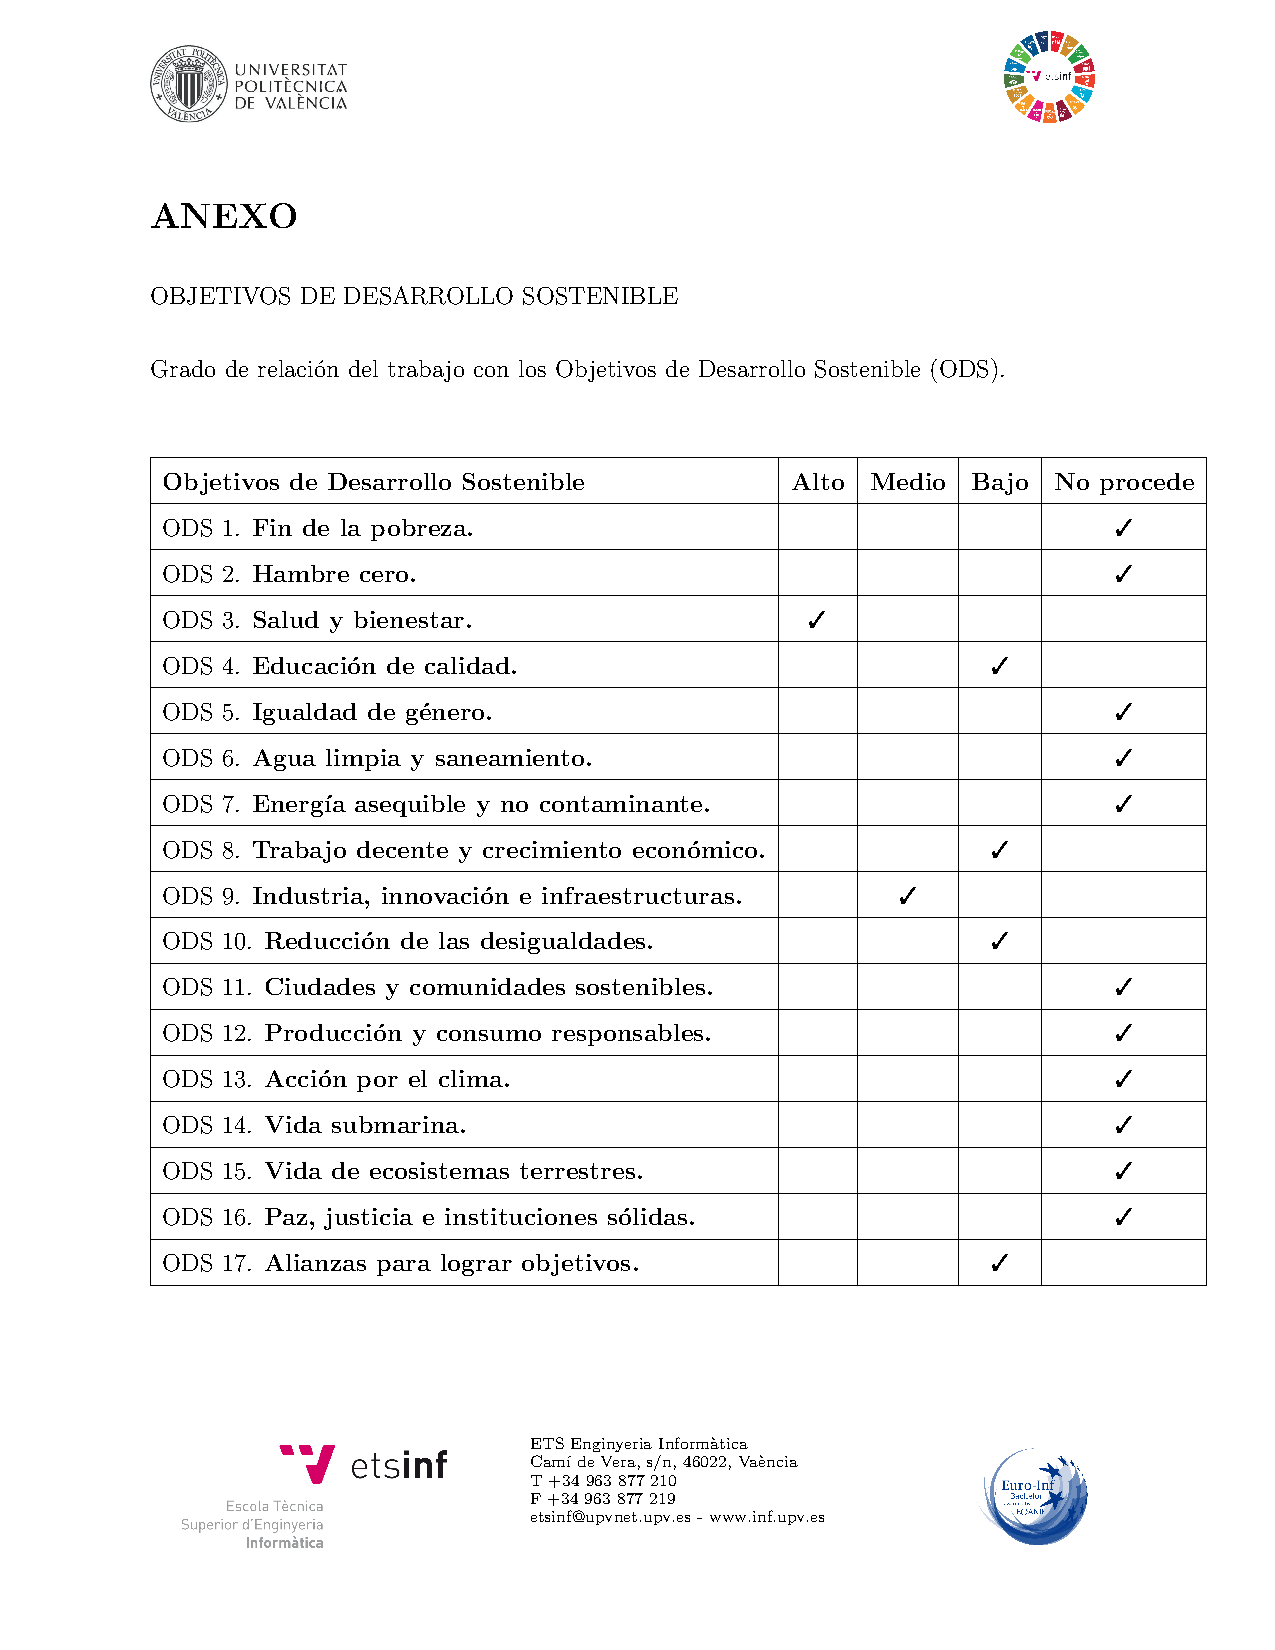
\includepdf[pages=-, pagecommand={}]{partes/Anexo_ODS_TFG.pdf}

%%%%%%%%%%%%%%%%%%%%%%%%%%%%%%%%%%%%%%%%%%%%%%%%%%%%%%%%%%%%%%%%%%%%%%%%%%%%%%%
%                              FI DEL DOCUMENT                                %
%%%%%%%%%%%%%%%%%%%%%%%%%%%%%%%%%%%%%%%%%%%%%%%%%%%%%%%%%%%%%%%%%%%%%%%%%%%%%%%

\end{document}
